\documentclass[3p,onecolumn]{elsarticle}

\usepackage{natbib}
\usepackage[version=4]{mhchem}
\usepackage{graphicx}
\journal{Fluid Phase Equilibria}

\bibliographystyle{elsarticle-num}
%%%%%%%%%%%%%%%%%%%%%%%

\begin{document}

\begin{frontmatter}

\title{Supporting material for ``A molecular dynamics study of the solvation of \ce{CO_2}, water, and some organic compounds in the ionic liquids \ce{[emim][B(CN)_4]} and \ce{[emim][NTf_2]}''}

%% Group authors per affiliation:
\author[rvt]{A.J.~Silveira}
\author[rvt]{S.~Pereda}
\author[focal,els]{F.W.~Tavares}
\author[focal]{C.R.A.~Abreu\corref{cor1}}
\ead{abreu@eq.ufrj.br}

\address[rvt]{Planta Piloto de Ingenier\'ia Qu\'imica, PLAPIQUI, Universidad Nacional del Sur,Camino La Carrindanga Km 7-CC: 717, Bah\'ia Blanca, Argentina}
\address[focal]{Chemical Engineering Department, Escola de Qu\'imica, Universidade Federal do Rio de Janeiro,Rio de Janeiro, RJ 21941-909, Brazil}
\address[els]{COPPE, Universidade Federal do Rio de Janeiro, Rio de Janeiro, RJ 21941-909, Brazil}

\cortext[cor1]{Corresponding author}
\end{frontmatter}

\begin{figure}[ht]
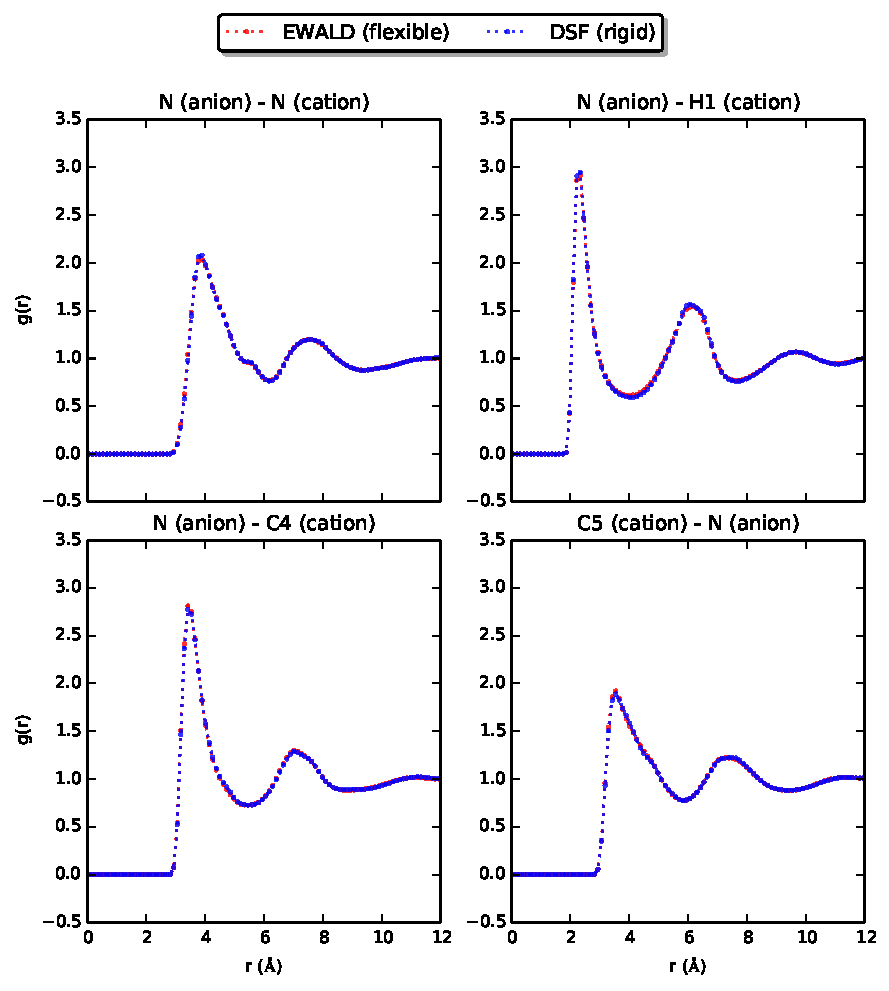
\includegraphics[]{rdf-koller}
\caption{\ce{[emim][B(CN)_4]}}
\label{fig:rdf-koller}
\end{figure}

\begin{figure}[ht]
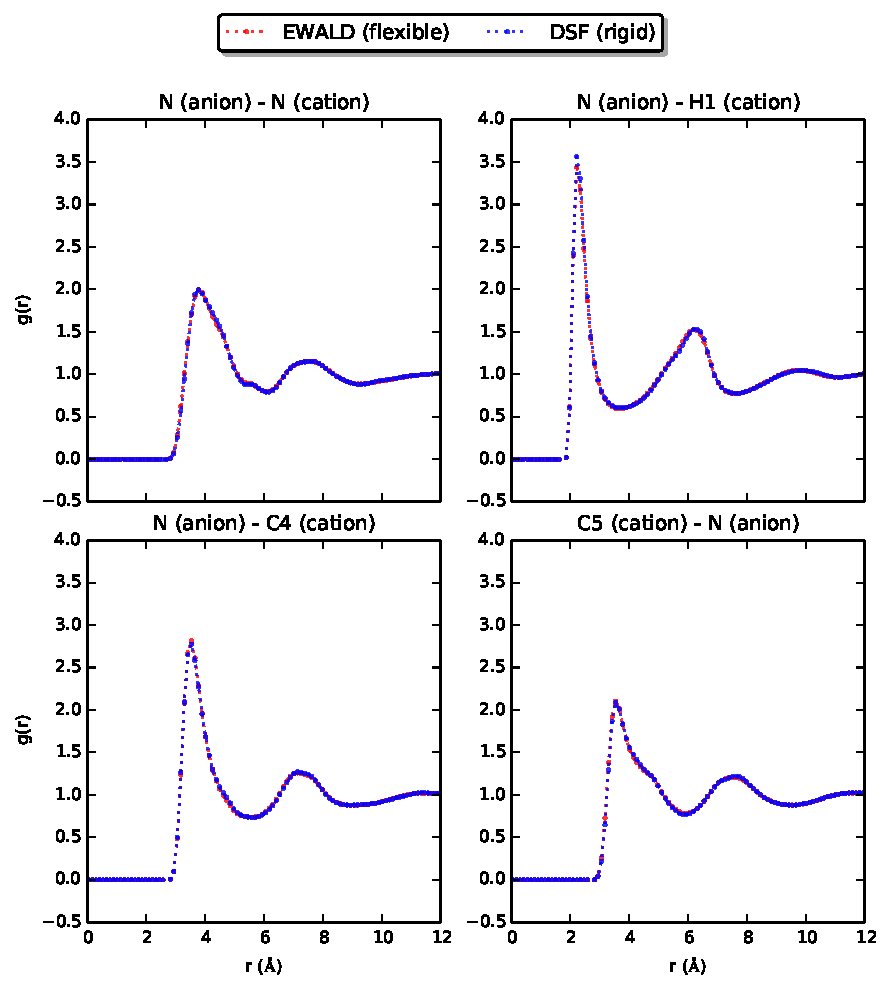
\includegraphics[]{rdf-Batista}
\caption{\ce{[emim][B(CN)_4]}}
\label{fig:rdf-Batista}
\end{figure}


\begin{figure}[ht]
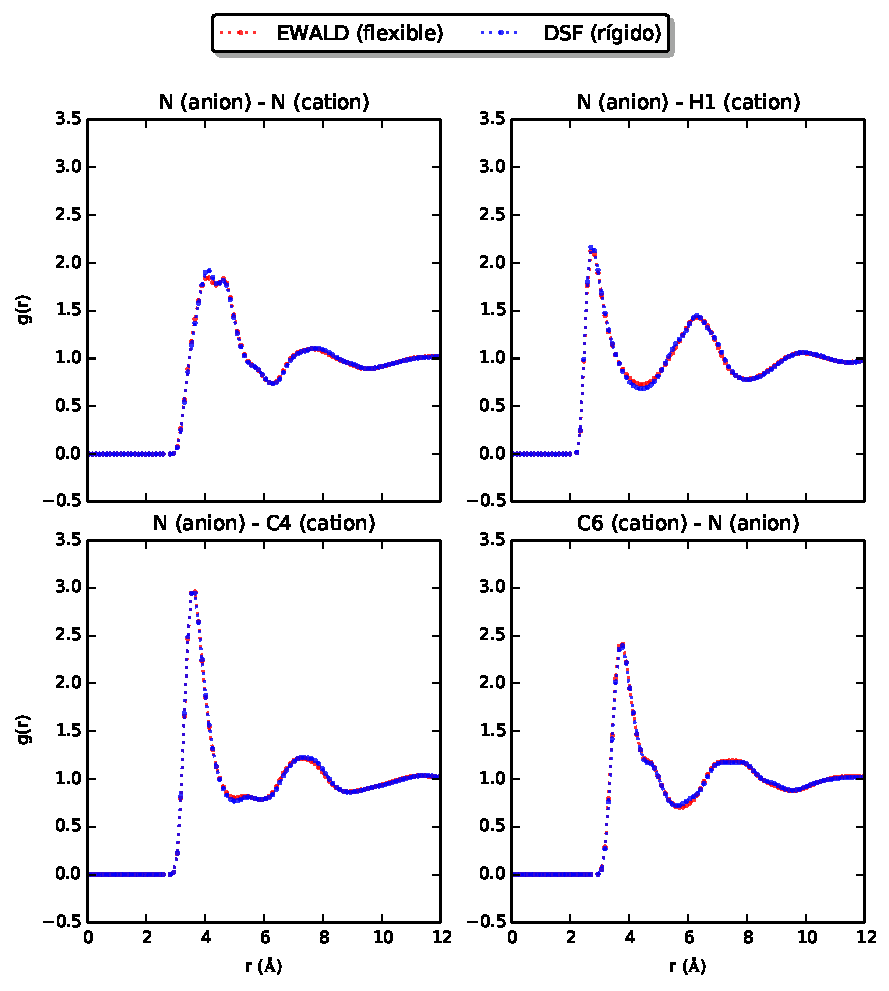
\includegraphics[]{rdf-Liu}
\caption{\ce{[emim][B(CN)_4]}}
\label{fig:rdf-Liu}
\end{figure}

\begin{figure}[ht]
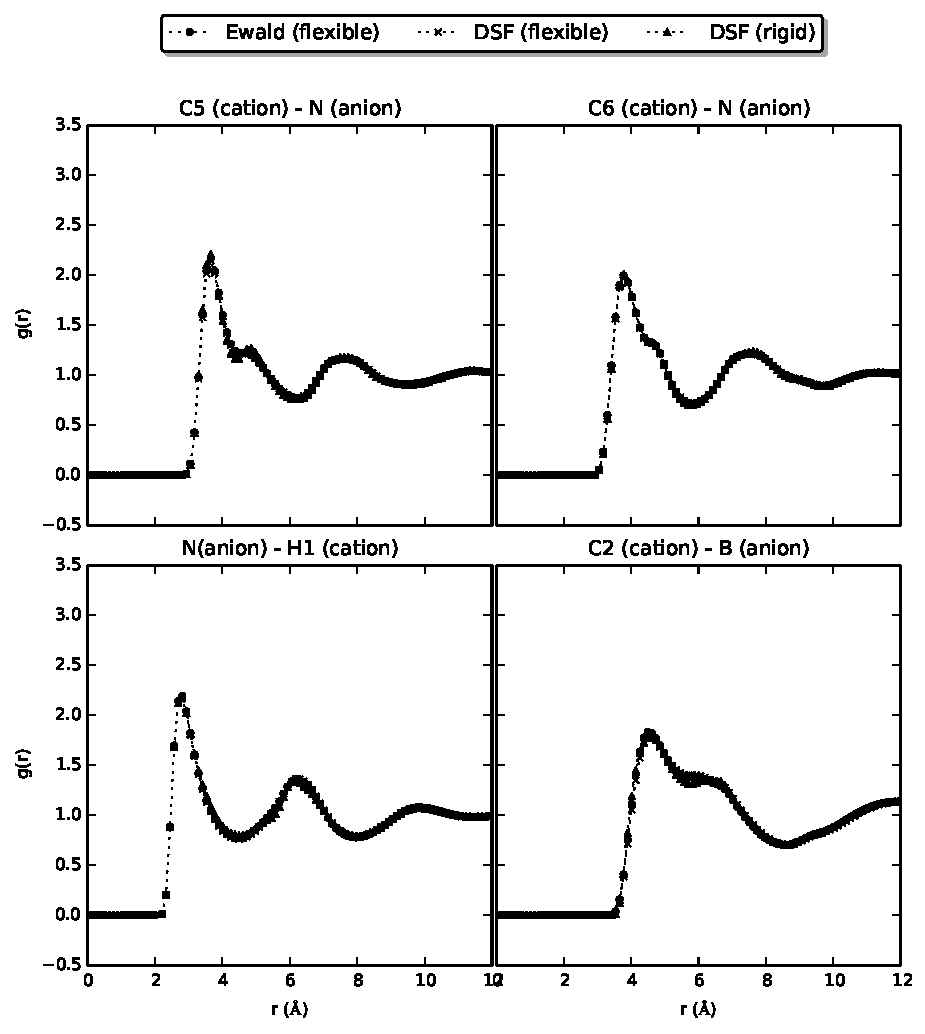
\includegraphics[]{rdf-Weber}
\caption{\ce{[emim][B(CN)_4]}}
\label{fig:rdf-Weber}
\end{figure}

\begin{figure}
	\centering
	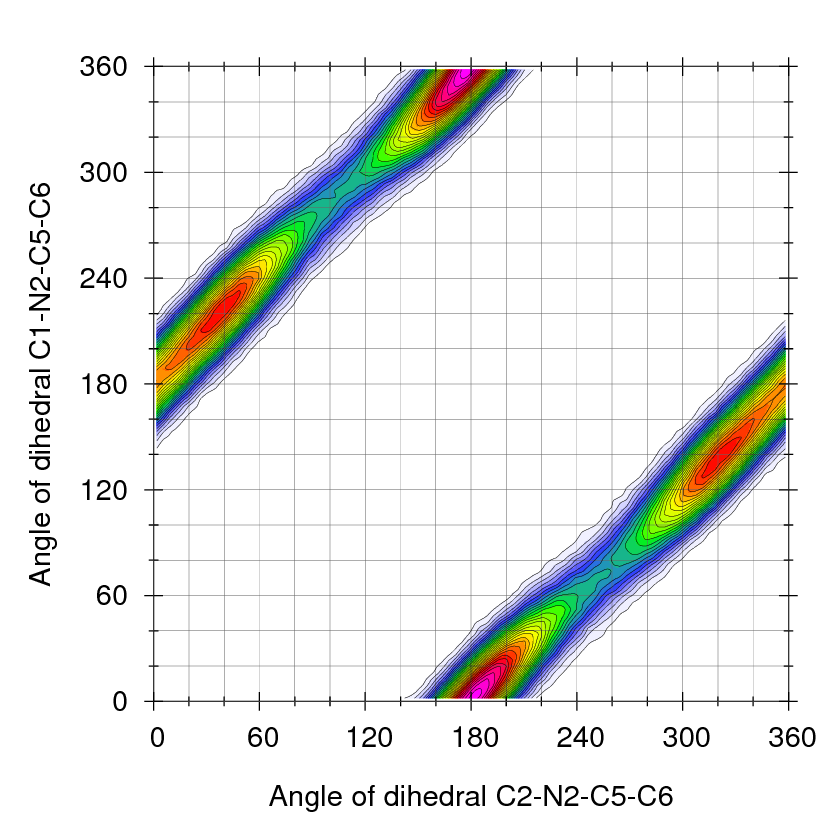
\includegraphics[width=\linewidth]{Ludwig}%
	
	%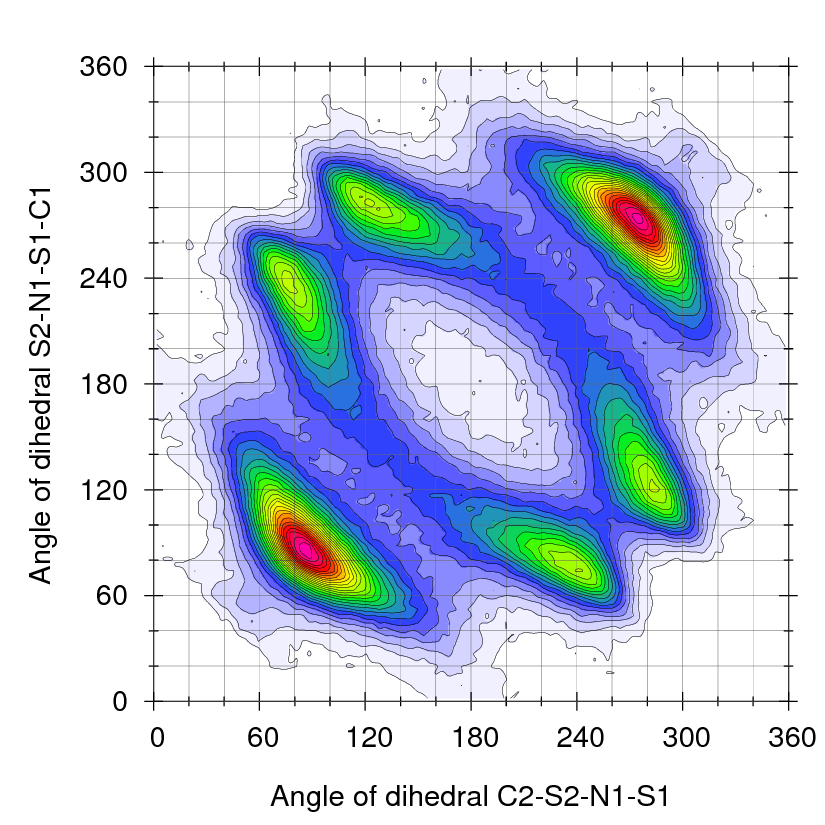
\includegraphics[width=\linewidth]{Ludwig_anion}%
	\caption{Combined distribution function of (a) the dihedral angles of C1-N2-C5-C6 and C2-N2-C5-C6, and (b) of the dihedral angles of the contiguous  C1-S1-N1-S2 and S1-N1-S2-C2 chains, obtained from NPT-MD simulations of 250 molecules of \ce{[emim][NTf_2]}.}
	\label{fig:die_ntf2}
\end{figure}

\end{document}